% RepNet Progress Update — Finalized Model Performance
% Same visual identity as final_presentation_modern.tex
% Compiles with pdfLaTeX.

\documentclass[10pt,aspectratio=169]{beamer}

% ====================
% Packages
% ====================
\usepackage[T1]{fontenc}
\usepackage{lmodern}
\usepackage{graphicx}
\usepackage{booktabs}
\usepackage{mathtools}
\usepackage{tikz}
\usetikzlibrary{positioning,arrows.meta}
\usepackage{hyperref}
\usepackage{pgfplots}
\pgfplotsset{compat=1.18}

% ====================
% UC Davis brand colors (digital palette)
% ====================
\definecolor{aggieblue}{HTML}{022851}
\definecolor{aggiegold}{HTML}{FFBF00}
\definecolor{aggieblueDark}{HTML}{011936}
\definecolor{aggiegoldDark}{HTML}{C99700}
\definecolor{coolgray}{RGB}{77,79,83}
\definecolor{boxgray}{RGB}{238,235,233}

% ====================
% Fonts
% ====================
\renewcommand{\familydefault}{\sfdefault}
\newcommand{\Raleway}{\sffamily}
\newcommand{\Lato}{\sffamily}

% ====================
% Beamer color slots
% ====================
\setbeamercolor*{palette primary}{fg=white,bg=aggieblue}
\setbeamercolor*{palette secondary}{fg=white,bg=coolgray}
\setbeamercolor*{palette tertiary}{fg=white,bg=aggieblueDark}
\setbeamercolor*{palette quaternary}{fg=aggieblue,bg=aggiegold}

\setbeamercolor{structure}{fg=aggieblue}
\setbeamercolor{titlelike}{fg=aggieblue}
\setbeamercolor{frametitle}{fg=white,bg=aggieblue}
\setbeamercolor{title}{fg=white,bg=aggieblue}
\setbeamercolor{author}{fg=aggieblue}
\setbeamercolor{institute}{fg=coolgray}
\setbeamercolor{date}{fg=coolgray}

\setbeamercolor{section in toc}{fg=aggieblue}
\setbeamercolor{subsection in toc}{fg=aggieblueDark}

% ====================
% Fonts (sizes/weights)
% ====================
\setbeamerfont{title}{family=\Raleway,series=\bfseries,size=\LARGE}
\setbeamerfont{subtitle}{family=\Lato,size=\normalsize}
\setbeamerfont{author}{family=\Lato,size=\small}
\setbeamerfont{institute}{family=\Lato,size=\footnotesize}
\setbeamerfont{date}{family=\Lato,size=\footnotesize}
\setbeamerfont{frametitle}{family=\Raleway,series=\bfseries,size=\large}
\setbeamerfont{section in toc}{family=\Raleway,series=\bfseries}
\setbeamerfont{subsection in toc}{family=\Lato,size=\small}
\setbeamerfont{footline}{family=\Lato,size=\scriptsize}

% ====================
% Frame title with Aggie Gold accent bar
% ====================
\setbeamertemplate{frametitle}{%
  \nointerlineskip
  \begin{beamercolorbox}[wd=\paperwidth,ht=3.0ex,dp=1.4ex,leftskip=1em,rightskip=1em]{frametitle}%
    \usebeamerfont{frametitle}\insertframetitle%
  \end{beamercolorbox}%
  \begin{beamercolorbox}[wd=\paperwidth,ht=0.35ex,dp=0pt]{palette quaternary}%
  \end{beamercolorbox}%
  \vspace{1.0ex}
}

\beamertemplatenavigationsymbolsempty

% ====================
% Table of Contents Customization
% ====================
\setbeamertemplate{section in toc}{\leavevmode\inserttocsection\par}

\setbeamertemplate{subsection in toc}{%
  \leavevmode\hspace{1.5em}%
  \color{aggiegoldDark}\raise0.4ex\hbox{\vrule width 0.4ex height 0.4ex}%
  \hspace{0.5em}\color{aggieblueDark}\inserttocsubsection\par
}

% ====================
% Footer
% ====================
\newcommand{\footercontent}[1]{\renewcommand{\insertfootercontent}{#1}}
\newcommand{\insertfootercontent}{}

\setbeamertemplate{footline}{%
  \ifx\insertfootercontent\@empty\else
    \begin{beamercolorbox}[wd=\paperwidth,ht=0.3ex,dp=0pt]{palette quaternary}\end{beamercolorbox}%
    \begin{beamercolorbox}[wd=\paperwidth,ht=2.4ex,dp=1.2ex,leftskip=1em,rightskip=1em]{palette primary}%
      \usebeamerfont{footline}\insertfootercontent\hfill\insertframenumber{}/\inserttotalframenumber%
    \end{beamercolorbox}%
  \fi
}

% ====================
% Title / authors
% ====================
\title{Risk Estimation of Preeclampsia}
\subtitle{}
\author{Ahmed Khan \and Lawrencedel Legaspi \and Selena Phu}
\institute{Department of Electrical and Computer Engineering \\ University of California, Davis}
\date{\today}

\titlegraphic{}

\footercontent{%
  \href{https://github.com/AhmedKhan-GH/repnet}{github.com/AhmedKhan-GH/repnet}
  \enspace$\bullet$\enspace
  UC Davis Senior Design 2026%
}

% ====================
% Title page template
% ====================
\setbeamertemplate{title page}{%
  \begin{tikzpicture}[remember picture,overlay]
    \fill[aggieblue]
      ([yshift=1cm]current page.north west)
      rectangle
      ([yshift=-3.8cm]current page.north east);
    \fill[aggiegold]
      ([yshift=-3.8cm]current page.north west)
      rectangle
      ([yshift=-3.95cm]current page.north east);
    \node[anchor=center,text=white,align=center,text width=10cm,
          font=\Raleway\bfseries]
      at ([yshift=-2.2cm]current page.north)
      {\usebeamerfont{title}\inserttitle};
    \node[anchor=center,text=aggiegold,align=center,text width=14cm,
          font=\Lato]
      at ([yshift=-2.4cm]current page.north)
      {\usebeamerfont{subtitle}\insertsubtitle};
    \node[anchor=north,text=aggieblue,align=center,font=\Lato]
      at ([yshift=-5.4cm]current page.north)
      {\usebeamerfont{author}\insertauthor};
    \node[anchor=north,text=coolgray,align=center,font=\Lato]
      at ([yshift=-6.0cm]current page.north)
      {\usebeamerfont{institute}\insertinstitute};
    \node[anchor=north,text=coolgray,align=center,font=\Lato]
      at ([yshift=-6.9cm]current page.north)
      {\usebeamerfont{date}\insertdate};
  \end{tikzpicture}%
}

% ====================
% 3D block drawing helper (x, y, width, height, depth, color)
% ====================
\newcommand{\tblock}[6]{%
  \pgfmathsetmacro{\tbw}{#3}\pgfmathsetmacro{\tbh}{#4}%
  \pgfmathsetmacro{\tbdx}{0.15*#5}\pgfmathsetmacro{\tbdy}{0.15*#5}%
  \fill[#6, opacity=0.8] (#1,#2) rectangle ++(#3,#4);
  \draw[#6!40!black] (#1,#2) rectangle ++(#3,#4);
  \fill[#6!75!white, opacity=0.6]
    (#1,{#2+#4}) -- ++(\tbdx,\tbdy) -- ++(#3,0) -- ++({-\tbdx},{-\tbdy}) -- cycle;
  \draw[#6!40!black]
    (#1,{#2+#4}) -- ++(\tbdx,\tbdy) -- ++(#3,0) -- ++({-\tbdx},{-\tbdy}) -- cycle;
  \fill[#6!55!black, opacity=0.5]
    ({#1+#3},#2) -- ++(\tbdx,\tbdy) -- ++(0,#4) -- ++({-\tbdx},{-\tbdy}) -- cycle;
  \draw[#6!40!black]
    ({#1+#3},#2) -- ++(\tbdx,\tbdy) -- ++(0,#4) -- ++({-\tbdx},{-\tbdy}) -- cycle;
}

% ====================
% Hidden section declarations to populate the TOC
% ====================
\section{Introduction}
\section{Decision-Tree Modeling}
\subsection{Dataset Profile}
\subsection{Feature Extraction}
\subsection{Feature Importance}
\subsection{Feature Selection Matrix}
\subsection{Baseline vs.\ Ensemble Performance}
\section{Neural Network Modeling}
\subsection{Preprocessing \& Training}
\subsection{Depthwise Separable Convolution}
\subsection{Squeeze-Excitation}
\subsection{Multi-Head Cross-Lead Attention}
\subsection{Model Performance}
\subsection{Interpretability}
\section{Conclusion}
\section{Future Work}


% ====================
% Document
% ====================
\begin{document}

% ---------- Title Slide ----------
{%
  \setbeamertemplate{footline}{}%
  \begin{frame}[plain,noframenumbering]
    \titlepage
  \end{frame}
}

% ---------- Table of Contents Slide ----------
\begin{frame}{Contents}
  \tableofcontents
\end{frame}

% ---------- Introduction Slide ----------
\begin{frame}{Introduction}
  \begin{columns}[T]

    \begin{column}{0.52\textwidth}
      \usebeamerfont{footline}\color{coolgray}
      {\small\Raleway\bfseries\color{aggieblue} What is Preeclampsia?}\\[0.3em]
      \begin{itemize}
        \item Pregnancy complication with dangerously high blood pressure and organ stress
        \item Typically develops after 20 weeks of gestation
        \item Can damage kidneys, liver, and brain --- may progress to eclampsia (seizures and coma)
        \item Currently diagnosed by symptoms that appear \textbf{late} (elevated BP, proteinuria)
      \end{itemize}

      \vspace{0.6em}
      {\small\Raleway\bfseries\color{aggieblue} Why ECG?}\\[0.3em]
      \begin{itemize}
        \item PE increases cardiac afterload --- leaves traces in the ECG waveform
        \item 12-lead ECG is routine, cheap, and already collected in prenatal care
        \item Goal: detect PE risk from the ECG \textbf{before} symptoms appear
      \end{itemize}
    \end{column}

    \begin{column}{0.44\textwidth}
      {\small\Raleway\bfseries\color{aggieblue} Our Approach}\\[0.3em]
      \usebeamerfont{footline}\color{coolgray}
      Two parallel modeling strategies on 2{,}178 ECG recordings (335 PE+, 1{,}843 PE$-$):\\[0.3em]

      \begin{beamercolorbox}[wd=\textwidth,rounded=true,leftskip=0.5em,rightskip=0.5em,sep=0.4em]{boxgray}
        \scriptsize\Lato\color{coolgray}
        \textbf{1.\ Decision-Tree Modeling}\\
        Handcrafted features (NeuroKit + MUSE) $\rightarrow$ feature selection $\rightarrow$ Random Forest \& ensemble classifiers
      \end{beamercolorbox}

      \vspace{0.4em}
      \begin{beamercolorbox}[wd=\textwidth,rounded=true,leftskip=0.5em,rightskip=0.5em,sep=0.4em]{boxgray}
        \scriptsize\Lato\color{coolgray}
        \textbf{2.\ Neural Network Modeling}\\
        Raw 12-lead waveform $\rightarrow$ RepNet-SE (depthwise-separable CNN + squeeze-excitation + cross-lead attention)
      \end{beamercolorbox}

      \vspace{0.4em}
      \begin{beamercolorbox}[wd=\textwidth,rounded=true,leftskip=0.5em,rightskip=0.5em,sep=0.3em]{boxgray}
        \scriptsize\Lato\color{coolgray}
        \textbf{Evaluation:} Patient-grouped cross-validation, StratifiedGroupKFold, 80/20 dev-test split
      \end{beamercolorbox}
    \end{column}

  \end{columns}
\end{frame}

% ---------- Transition Slide ----------
{%
  \setbeamertemplate{footline}{}%
  \begin{frame}[plain,noframenumbering]
    \begin{tikzpicture}[remember picture,overlay]
      \fill[aggieblue] (current page.south west) rectangle (current page.north east);
    \end{tikzpicture}
    \vfill
    \centering
    {\Raleway\bfseries\Huge\color{white} Decision-Tree Modeling}\\[0.6em]
    {\color{aggiegold}\rule{6cm}{0.06cm}}
    \vfill
  \end{frame}
}

% ---------- Subsection Slide: Dataset Profile ----------
\begin{frame}{Decision-Tree Modeling --- Dataset Profile}
  \begin{columns}[T]
    
    % Left Column: Cohort Breakdown Table & Details
    \begin{column}{0.50\textwidth}
      \centering
      {\small\Raleway\bfseries\color{aggieblue} ECG Dataset}\\[0.4em]
      \resizebox{\textwidth}{!}{%
        \begin{tabular}{lccc}
          \toprule
          \textbf{Dataset} & \textbf{\shortstack{Original Total\\(Preeclamptic/Normal)}} & \textbf{\shortstack{Dropped ECGs\\(Preeclamptic/Normal)}} & \textbf{\shortstack{Final Total\\(Preeclamptic/Normal)}} \\
          \midrule
          Unbalanced & 337 / 1854 & 8 / 24 & 329 / 1830 \\
          Balanced   & 187 / 182  & 6 / 1  & 181 / 181 \\
          \bottomrule
        \end{tabular}
      }%
      
      \vspace{0.8em}
      \begin{flushleft}
        \usebeamerfont{footline}\color{coolgray}
        \textbf{MUSE Diagnostics:} This dataset includes a structured metadata CSV containing \textbf{656 distinct features}.
        
        \vspace{0.4em}
        \textbf{Exclusion Criteria:} Samples dropped due to:
        \begin{itemize}
          \item Delineation issues using certain cleaning methods for each lead within \textbf{NeuroKit} framework.
          \item Empty data within a lead.
        \end{itemize}
      \end{flushleft}
    \end{column}
    
    % Right Column: Preprocessed Lead Signal Image
    \begin{column}{0.46\textwidth}
      \centering
      {\small\Raleway\bfseries\color{aggieblue} Lead Visualizations}\\[0.4em]
      \begin{beamercolorbox}[wd=\textwidth,rounded=true,shadow=false,leftskip=0.2em,rightskip=0.2em,sep=0.2em]{boxgray}
        \centering
        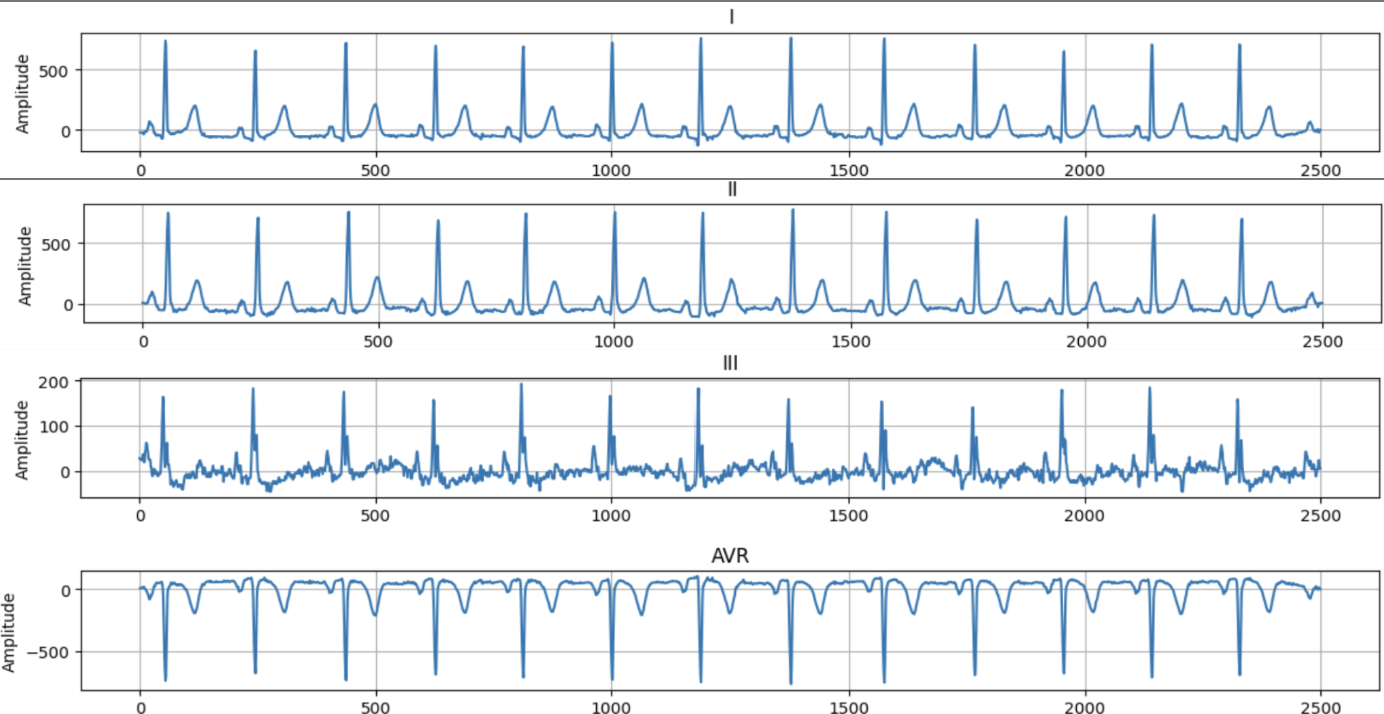
\includegraphics[width=0.96\textwidth,height=3.8cm,keepaspectratio]{4leadsexample.png}
      \end{beamercolorbox}
      \vspace{0.3em}
      {\scriptsize\Lato\color{coolgray} Representative trace behavior of select isolated signal leads (e.g., I, II, III, aVR) after preprocessing filters are applied.}
    \end{column}

  \end{columns}
\end{frame}

% ---------- Subsection Slide: Feature Extraction ----------
\begin{frame}{Decision-Tree Modeling --- Feature Extraction}
  \begin{columns}[T]
    
    % Left Column: Neurokit Feature Pipeline
    \begin{column}{0.48\textwidth}
      \centering
      {\small\Raleway\bfseries\color{aggieblue} Neurokit ECG Features}\\[0.4em]
      \resizebox{\textwidth}{!}{%
        \begin{tabular}{ll}
          \toprule
          \textbf{Feature} & \textbf{Equation} \\
          \midrule
          $P_{\max}$ & $\max_{\ell \in \mathcal{L}}(P_{\text{off}}^{\ell} - P_{\text{on}}^{\ell})$ \\
          $P_{\min}$ & $\min_{\ell \in \mathcal{L}}(P_{\text{off}}^{\ell} - P_{\text{on}}^{\ell})$ \\
          P-Wave Disp. & $P_{\max} - P_{\min}$ \\
          QT Dispersion & $QT_{\max} - QT_{\min}$ \\
          $T_{pe}$ Interval & $\text{mean}(T_{\text{off}} - T_{\text{peak}})$ \\
          $T_{pe}/\text{QT}$ & $T_{pe} \text{ Interval} / \text{mean}(T_{\text{off}} - R_{\text{on}})$ \\
          $T_{pe}/\text{QTc}$ & $(T_{pe}/\text{QT}) / \sqrt{\text{mean}(\Delta R_{\text{peak}})}$ \\
          ST Elevation & $\boldsymbol{1} \text{ if } > 50\%\text{ elevated, } \boldsymbol{0}\text{ otherwise}$ \\
          ST Depression & $\boldsymbol{1} \text{ if } > 50\%\text{ depressed, } \boldsymbol{0}\text{ otherwise}$ \\
          Avg. Amp. Diff. & $\text{mean}(A_{\text{ST}} - A_{\text{PR}})$ \\
          Med. Amp. Diff. & $\text{med}(A_{\text{ST}} - A_{\text{PR}})$ \\
          Max. Amp. Diff. & $\max(A_{\text{ST}} - A_{\text{PR}})$ \\
          Min. Amp. Diff. & $\min(A_{\text{ST}} - A_{\text{PR}})$ \\
          Frontal QRS-T & $|\text{QRS Axis} - \text{T Axis}|$ \\
          \bottomrule
        \end{tabular}
      }%
    \end{column}
    
    % Right Column: MUSE Feature Pipeline + Footnote Text (Clean & Compact)
    \begin{column}{0.48\textwidth}
      \centering
      {\small\Raleway\bfseries\color{aggieblue} MUSE-derived Features}\\[0.4em]
      \resizebox{\textwidth}{!}{%
        \begin{tabular}{ll}
          \toprule
          \textbf{Feature} & \textbf{Equation} \\
          \midrule
          $P_{\max}$ & $\max(\text{P\_Duration for 12 leads})$ \\
          $P_{\min}$ & $\min(\text{P\_Duration for 12 leads})$ \\
          P-Wave Disp. & $P_{\max} - P_{\min}$ \\
          QT Dispersion & $QT = \sum \text{comp. durations} + \frac{1}{8}RR; \, \max(QT) - \min(QT)$ \\
          $T_{pe}$ Interval & $\text{T\_Duration} + \text{T\_PrimeDuration} - \text{STEtoTPeak}$ \\
          $T_{pe}/\text{QT}$ & $T_{pe} \text{ Interval} / \text{QT}$ \\
          $T_{pe}/\text{QTc}$ & $T_{pe}/\text{QT} \cdot \sqrt{RR}$ \\
          ST Elevation & $(\text{BITFLGS} \ \& \ 8) \neq 0$ \\
          ST Depression & $(\text{BITFLGS} \ \& \ 4) \neq 0$ \\
          QRS Axis & $\text{RAxis from metadata}$ \\
          T Axis & $\text{TAxis from metadata}$ \\
          Frontal QRS-T & $|\text{QRS Axis} - \text{T Axis}|$ \\
          \bottomrule
        \end{tabular}
      }%
      
      \vspace{1.2em}
      \begin{beamercolorbox}[wd=\textwidth,rounded=true,shadow=false,leftskip=0.6em,rightskip=0.6em,sep=0.4em]{boxgray}
        \usebeamerfont{footline}\color{coolgray}
        \textbf{Implementation Note:} We extracted QRS and T Axis in Neurokit, though we do not have a definite equation.
      \end{beamercolorbox}
    \end{column}

  \end{columns}
\end{frame}

% ---------- Subsection Slide: Model Performance ----------
\begin{frame}{Decision-Tree Modeling --- Feature Importance}
  \centering
  {\small\Raleway\bfseries\color{aggieblue} Random Forest Performance}\\[0.3em]
  
  \resizebox{0.95\textwidth}{!}{%
    \begin{tabular}{lcccccccc}
      \toprule
      \textbf{Method} & \textbf{\# Features} & \textbf{AUROC} & \textbf{AUPRC} & \textbf{Specificity} & \textbf{Sensitivity} & \textbf{Bal. Accuracy} & \textbf{Precision} & \textbf{F1-Score} \\
      \midrule
      Original & 723 & $69.93 \pm 3.30$ & $32.55 \pm 3.71$ & $73.74 \pm 3.26$ & $56.12 \pm 8.60$ & $64.93 \pm 3.71$ & $27.97 \pm 2.62$ & $37.20 \pm 3.89$ \\
      Pearson Corr. & 363 & $70.97 \pm 3.86$ & $35.14 \pm 7.29$ & $74.57 \pm 4.37$ & $54.89 \pm 3.83$ & $64.73 \pm 2.62$ & $28.64 \pm 4.02$ & $37.45 \pm 3.48$ \\
      \textbf{ANOVA} & \textbf{191} & $\mathbf{74.54 \pm 3.88}$ & $\mathbf{37.71 \pm 5.03}$ & $74.15 \pm 3.08$ & $\mathbf{62.04 \pm 10.59}$ & $\mathbf{68.10 \pm 4.37}$ & $\mathbf{30.08 \pm 2.62}$ & $\mathbf{40.36 \pm 4.10}$ \\
      RFECV & 175 & $73.31 \pm 3.77$ & $38.12 \pm 6.08$ & $74.48 \pm 2.73$ & $59.32 \pm 10.49$ & $66.90 \pm 3.96$ & $29.30 \pm 1.61$ & $39.08 \pm 3.60$ \\
      \midrule
      Intersection & 176 & $73.09 \pm 4.43$ & $36.58 \pm 7.34$ & $73.06 \pm 4.90$ & $61.15 \pm 14.82$ & $71.24 \pm 2.02$ & $28.75 \pm 1.54$ & $38.76 \pm 4.25$ \\
      \bottomrule
    \end{tabular}
  }%

  \vspace{0.6em}
  \begin{beamercolorbox}[wd=0.95\textwidth,rounded=true,leftskip=0.8em,rightskip=0.8em,sep=0.4em]{boxgray}
    \usebeamerfont{footline}\color{coolgray}
    \textbf{Performance Insight:} Features chosen \textbf{sequentially} yielded stronger performance results compared to doing the importances \textbf{individually} and intersecting the common features.
  \end{beamercolorbox}
\end{frame}

% ---------- Subsection Slide: Feature Importance Breakdown ----------
\begin{frame}{Decision-Tree Modeling --- Feature Importance}
  \begin{columns}[T]
    
    % Left Column: Methodological Framework details
    \begin{column}{0.42\textwidth}
      \usebeamerfont{footline}\color{coolgray}
      \textbf{Cross-Validation Strategy:}
      \begin{itemize}
        \item\textbf{StratifiedGroupKFold} with 5 folds grouped by the Patient's MRN
        \item\textbf{RandomForest} with \textbf{RandomUnderSampler} inside the folds
      \end{itemize}

      \vspace{0.2em}
      \textbf{Feature Selection:}
      \begin{itemize}
        \item \textbf{Pearson Correlation:} Drops one feature out of colinear pairs sharing a correlation value $> 0.85$.
        \item \textbf{ANOVA (Analysis of Variance):} Keeps features with $p < 0.05$.
        \item \textbf{RFECV:} Used roc\_auc scoring to recursively remove features
      \end{itemize}
      
      \vspace{0.2em}
      \begin{beamercolorbox}[wd=\textwidth,rounded=true,leftskip=0.5em,rightskip=0.5em,sep=0.3em]{boxgray}
        \scriptsize\Lato\color{coolgray}
        \textbf{Hindsight Note:} Evaluating RFECV on \textit{average\_precision} or \textit{balanced\_accuracy} may have been better for the primary goal of detecting preeclampsia.
      \end{beamercolorbox}
    \end{column}
    
    % Right Column: Lead distribution chart
    \begin{column}{0.54\textwidth}
      \centering
      {\small\Raleway\bfseries\color{aggieblue} Feature Counts Across Leads}\\[0.3em]
      \begin{beamercolorbox}[wd=\textwidth,rounded=true,leftskip=0.1em,rightskip=0.1em,sep=0.1em]{boxgray}
        \centering
        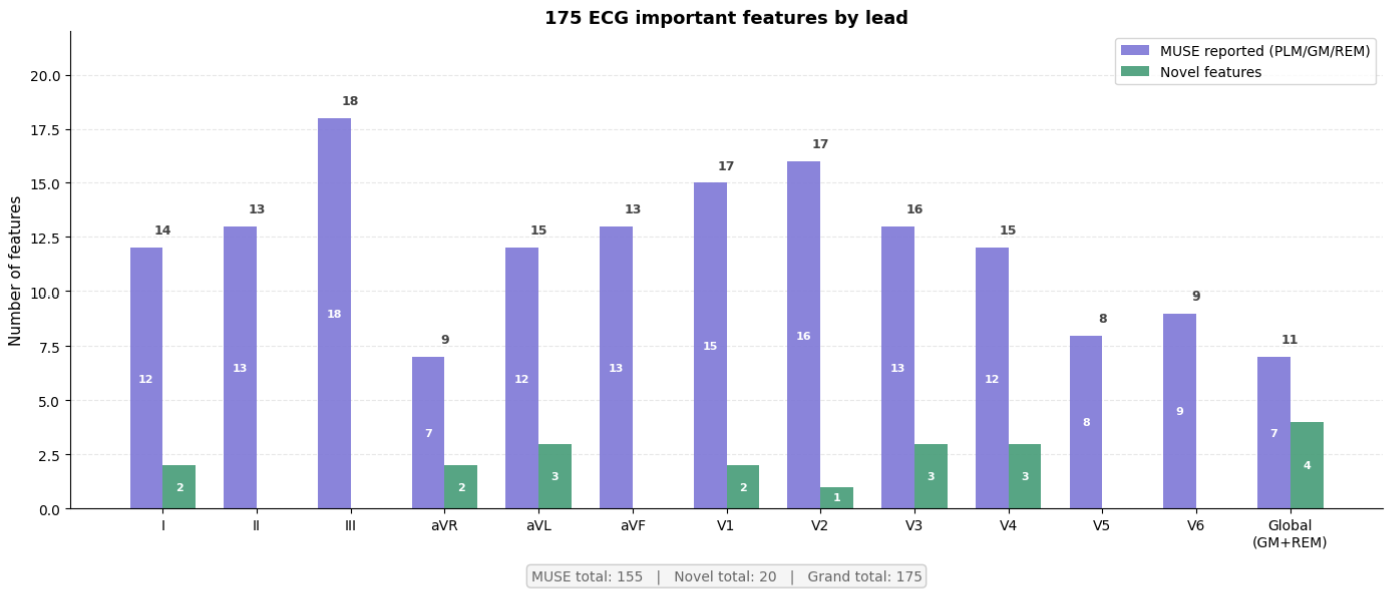
\includegraphics[width=0.98\textwidth,height=4.2cm,keepaspectratio]{leadimportance.png}
      \end{beamercolorbox}
      \vspace{0.4em}
      \begin{flushleft}
        \usebeamerfont{footline}\color{coolgray}
        \textbf{Lead Significance:} Graph maps feature distribution counts across different leads, showing which leads may be more important.
      \end{flushleft}
    \end{column}

  \end{columns}
\end{frame}

% ---------- Subsection Slide: Feature Selection Matrix ----------
\begin{frame}{Decision-Tree Modeling --- Multi-Metric Selection Matrix}
  
  % [onlytextwidth] removes outer margins to give the wide heatmap maximum breathing room
  \begin{columns}[c, onlytextwidth] 
    
    % Left Column: Maximized Heatmap Allocation (82% width)
    \begin{column}{0.82\textwidth}
      \centering
      {\small\Raleway\bfseries\color{aggieblue} Feature Selection by Methods --- 12 Leads}\\[0.3em]
      \begin{beamercolorbox}[wd=\textwidth,rounded=true,leftskip=0.1em,rightskip=0.1em,sep=0.1em]{boxgray}
        \centering
        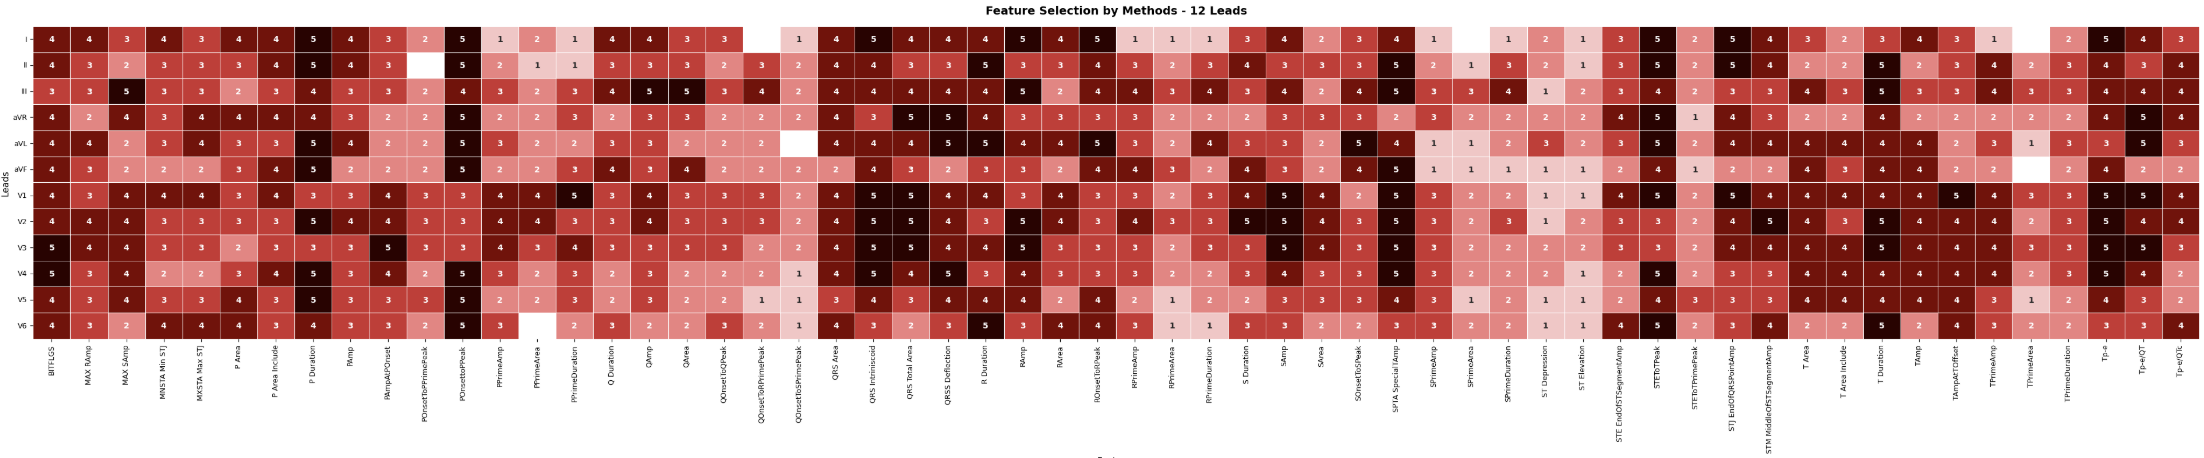
\includegraphics[width=\textwidth,height=4.2cm,keepaspectratio]{Heatmap12lead2.png}
      \end{beamercolorbox}
    \end{column}
    
    % Right Column: Downsized Legend Allocation (15% width)
    \begin{column}{0.15\textwidth}
      \centering
      \vspace{1.2em} % Subtle vertical alignment adjustment
      \begin{beamercolorbox}[wd=\textwidth,rounded=true,leftskip=0.1em,rightskip=0.1em,sep=0.1em]{boxgray}
        \centering
        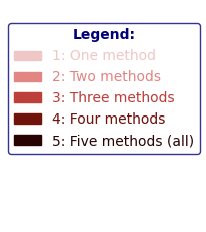
\includegraphics[width=\textwidth,keepaspectratio]{heatmaplegend.png}
      \end{beamercolorbox}
    \end{column}

  \end{columns}

  \vspace{0.6em}
  \rule{\textwidth}{0.4pt}

  % Contextual Breakdown spanning beneath the images
  \begin{columns}[T, onlytextwidth]
    \begin{column}{0.48\textwidth}
      \usebeamerfont{footline}\color{coolgray}
      \textbf{Feature Selection Methods:} Previous Pearson, ANOVA, and RFECV (roc\_auc), but now includes RFECV (balanced\_accuracy and average\_precision)
    \end{column}
    \begin{column}{0.48\textwidth}
      \usebeamerfont{footline}\color{coolgray}
      \textbf{Pipeline Constraint Note:} The additional balanced\_accuracy and average\_precision are not included for the future ensemble modeling as these were included afterwards. This heatmap is just a showing of how important overall features may be and can tell us whether a feature is universally important across leads.
    \end{column}
  \end{columns}
\end{frame}

% ---------- Subsection Slide: Final Sequential Feature Importance ----------
\begin{frame}{Decision-Tree Modeling --- Final Feature Importance}
  \begin{columns}[T]
    
    % Left Column: Deep Dive into the exact features you called out
    \begin{column}{0.44\textwidth}
      \usebeamerfont{footline}\color{coolgray}
      \textbf{Key Predictor Breakdown:}
      \begin{itemize}
        \item \textbf{Highest seen Features:} \texttt{BITFLGS}, \texttt{QRS Intrinsicoid}, and \texttt{STEtoTPeak} were most frequent across the 12-lead array.
        \item \textbf{NeuroKit Local Features:} The most critical lead-isolated extractors were \textbf{Tp-e}, \textbf{Tp-e/QT}, and \textbf{ST Depression}.
        \item \textbf{Surviving Global Features:} Beyond individual leads, the non-isolated features that cleared selection were \textbf{$P_{\max}$}, \textbf{$P_{\min}$}, \textbf{T Axis}, and the \textbf{Frontal QRS-T Angle}.
      \end{itemize}
    \end{column}
    
    % Right Column: The Sequential Feature Importance Bar Chart
    \begin{column}{0.54\textwidth}
      \centering
      {\small\Raleway\bfseries\color{aggieblue} Final Active Modeling Features}\\[0.3em]
      \begin{beamercolorbox}[wd=\textwidth,rounded=true,leftskip=0.1em,rightskip=0.1em,sep=0.1em]{boxgray}
        \centering
        % Generates the horizontal bar chart mapping counts/importance from sequential selection
        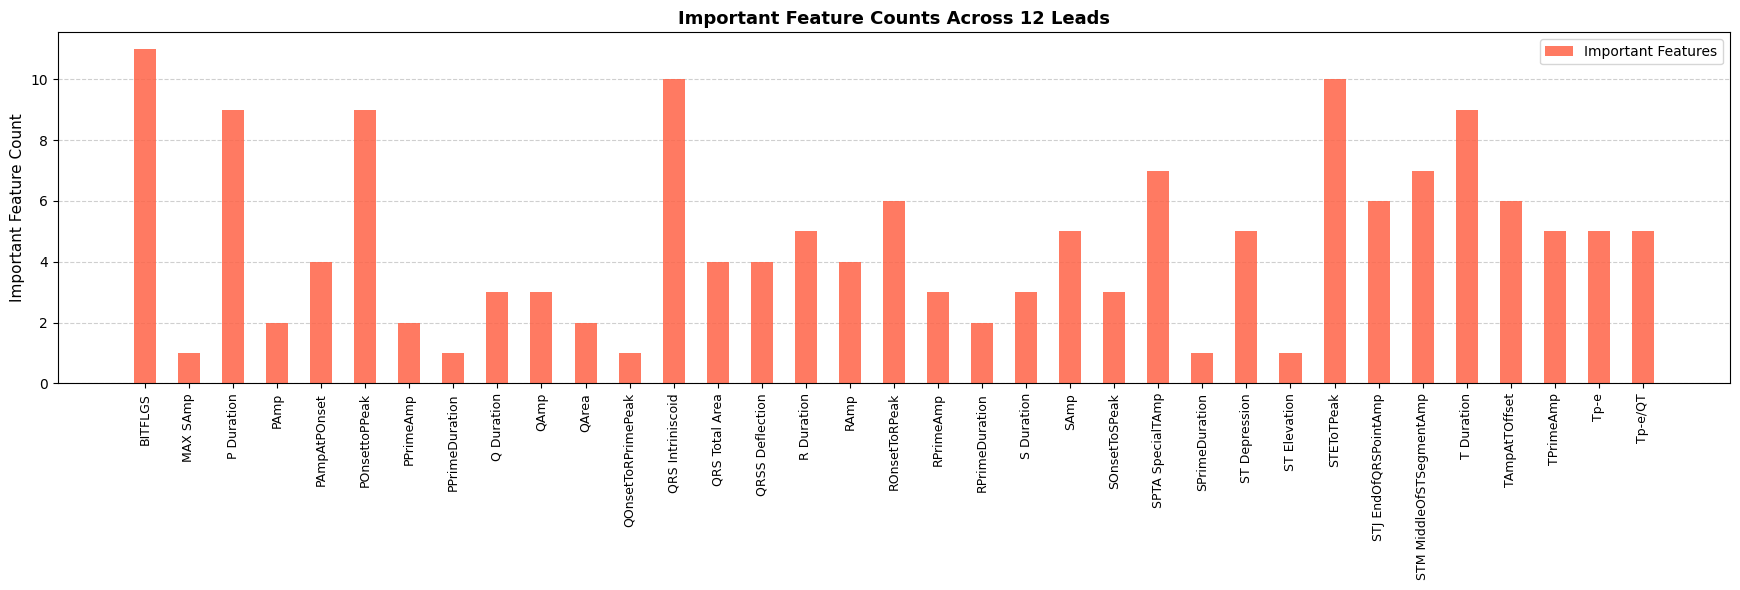
\includegraphics[width=0.98\textwidth,height=3.8cm,keepaspectratio]{featureimportance.png}
      \end{beamercolorbox}
      \vspace{0.3em}
      \begin{flushleft}
        \usebeamerfont{footline}\color{coolgray}
        \textbf{This distribution} shows the final feature space pruned through the Pearson $\rightarrow$ ANOVA $\rightarrow$ RFECV sequential chain.
      \end{flushleft}
    \end{column}

  \end{columns}
\end{frame}

% ---------- Subsection Slide: Model Performance Comparison ----------
\begin{frame}{Decision-Tree Modeling --- Baseline vs. Ensemble Performance}
  
  % Tighten padding slightly to give the text boxes maximum horizontal clearance
  \setlength{\tabcolsep}{3.5pt}
  
  \begin{columns}[T, onlytextwidth]
    
    % Left Column: Custom Commentary Text Box Placeholder (34% width)
    \begin{column}{0.34\textwidth}
      \vspace{0.2em}
      \begin{beamercolorbox}[wd=\textwidth,rounded=true,leftskip=0.8em,rightskip=0.8em,sep=0.8em]{boxgray}
        
        \usebeamerfont{footline}\color{coolgray}
        
     
        \textbf{Model Observations:}
        \begin{itemize}
          \item placeholder
          \item placeholder
          \item placeholder
        \end{itemize}
        
      \end{beamercolorbox}
    \end{column}
    
    % Right Column: Fixed Native LaTeX Performance Tables (63% width)
    \begin{column}{0.63\textwidth}
      \centering
      
      % Top Section: Standalone Base Models Table
      {\scriptsize\Raleway\bfseries\color{aggieblue} Standalone Tree-Based Classifiers}\\[0.3em]
      \begin{beamercolorbox}[wd=\textwidth,rounded=true,leftskip=0.2em,rightskip=0.2em,sep=0.4em]{boxgray}
        \tiny
        % \resizebox ensures the table never clips past the gray container boundaries
        \resizebox{\textwidth}{!}{
          \begin{tabular}{lcccccc}
            \textbf{Model} & \textbf{AUROC} & \textbf{AUPRC} & \textbf{Specificity} & \textbf{Sensitivity} & \textbf{Balanced Accuracy} & \textbf{F1-Score} \\
            \hline
            RandomForest & $74.49 \pm 3.77$ & $42.56 \pm 7.60$ & $74.37 \pm 3.20$ & $61.43 \pm 11.36$ & $67.90 \pm 4.30$ & $40.10 \pm 3.86$ \\
            LightGBM     & $73.25 \pm 3.47$ & $37.30 \pm 7.47$ & $72.95 \pm 4.33$ & $59.62 \pm 9.49$  & $66.28 \pm 2.62$ & $38.24 \pm 1.88$ \\
            XGBoost      & $74.84 \pm 4.50$ & $40.76 \pm 7.14$ & $74.26 \pm 3.76$ & $61.44 \pm 11.11$ & $67.85 \pm 4.28$ & $40.09 \pm 3.93$ \\
            CatBoost     & $74.55 \pm 4.94$ & $42.24 \pm 8.67$ & $75.96 \pm 4.81$ & $60.53 \pm 13.37$ & $68.24 \pm 4.56$ & $41.70 \pm 3.90$ \\
            AdaBoost     & $69.86 \pm 4.43$ & $33.91 \pm 7.71$ & $67.92 \pm 7.96$ & $59.90 \pm 13.17$ & $63.91 \pm 3.04$ & $35.14 \pm 2.44$ \\
          \end{tabular}
        }
      \end{beamercolorbox}
      
      \vspace{0.6em}
      
      % Bottom Section: Ensemble Architectures Table
      {\scriptsize\Raleway\bfseries\color{aggieblue} Multi-Model Ensemble Frameworks}\\[0.3em]
      \begin{beamercolorbox}[wd=\textwidth,rounded=true,leftskip=0.2em,rightskip=0.2em,sep=0.4em]{boxgray}
        \tiny
        \resizebox{\textwidth}{!}{
          \begin{tabular}{lcccccc}
            \textbf{Ensemble} & \textbf{AUROC} & \textbf{AUPRC} & \textbf{Specificity} & \textbf{Sensitivity} & \textbf{Balanced Accuracy} & \textbf{F1-Score} \\
            \hline
            Unweighted Voting  & $74.54 \pm 4.16$ & $41.81 \pm 7.86$ & $74.26 \pm 3.95$ & $59.32 \pm 10.70$ & $66.79 \pm 3.60$ & $38.94 \pm 2.99$ \\
            Weighted Voting    & $74.75 \pm 4.48$ & $42.26 \pm 7.92$ & $74.75 \pm 4.48$ & $60.23 \pm 10.88$ & $67.49 \pm 3.45$ & $39.80 \pm 2.76$ \\
            \textbf{Unweighted Voting+} & $\mathbf{75.72 \pm 3.94}$ & $41.58 \pm 8.03$ & $74.64 \pm 4.70$ & $\mathbf{62.35 \pm 10.93}$ & $\mathbf{68.50 \pm 3.22}$ & $40.85 \pm 2.24$ \\
            Stacking           & $74.77 \pm 4.35$ & $42.43 \pm 7.59$ & $74.37 \pm 4.18$ & $59.62 \pm 10.80$ & $67.00 \pm 3.46$ & $39.17 \pm 2.79$ \\
            Bagging CatBoost   & $74.81 \pm 4.98$ & $41.96 \pm 8.86$ & $74.70 \pm 4.68$ & $59.62 \pm 15.19$ & $67.16 \pm 5.59$ & $39.10 \pm 5.21$ \\
          \end{tabular}
        }
      \end{beamercolorbox}
      
    \end{column}

  \end{columns}
\end{frame}

% ==========================================================================
% CNN / TRANSFORMER ARCHITECTURE SECTION
% ==========================================================================

% ---------- Transition Slide: Neural Network Modeling ----------
{%
  \setbeamertemplate{footline}{}%
  \begin{frame}[plain,noframenumbering]
    \begin{tikzpicture}[remember picture,overlay]
      \fill[aggieblue] (current page.south west) rectangle (current page.north east);
    \end{tikzpicture}
    \vfill
    \centering
    {\Raleway\bfseries\Huge\color{white} Neural Network Modeling}\\[0.6em]
    {\color{aggiegold}\rule{6cm}{0.06cm}}
    \vfill
  \end{frame}
}

% ---------- Subsection Slide: Preprocessing & Training ----------
\begin{frame}{Neural Network Modeling --- Preprocessing \& Training}
  \begin{columns}[T]

    \begin{column}{0.48\textwidth}
      \centering
      {\small\Raleway\bfseries\color{aggieblue} Signal Preprocessing}\\[0.4em]
      \usebeamerfont{footline}\color{coolgray}
      Three steps applied per-lead in order:
      \begin{enumerate}
        \item \textbf{Baseline Wander Removal:} 4th-order Butterworth high-pass at 0.5~Hz, zero-phase SOS form
        \item \textbf{Powerline Interference:} 60~Hz IIR notch filter ($Q=30$); notch width $\sim$1~Hz
        \item \textbf{Z-Score Normalization:} Per-lead $\frac{x - \mu_\ell}{\sigma_\ell + \epsilon}$
      \end{enumerate}

      \vspace{0.4em}
      {\small\Raleway\bfseries\color{aggieblue} 7-Transform On-the-Fly Augmentation}\\[0.3em]
      \resizebox{\textwidth}{!}{%
        \begin{tabular}{lll}
          \toprule
          \textbf{Transform} & \textbf{Probability} & \textbf{Range} \\
          \midrule
          Gaussian Noise & 50\% & $\sigma \in [0.01, 0.05]$ \\
          Amplitude Scale & 50\% & $\pm 15\%$ \\
          Time Shift & 30\% & $\pm 150$ samples \\
          Lead Dropout & 10\% & 12\% per lead \\
          Cutout & 25\% & 50--200 samples \\
          Baseline Wander & 20\% & 0.05--0.5~Hz \\
          Speed Perturb & 10\% & $\pm 5\%$ \\
          \bottomrule
        \end{tabular}
      }%
      \vspace{0.2em}
      {\scriptsize\Lato\color{coolgray} Applied stochastically per sample during training. Class balance via \textbf{WeightedRandomSampler}.}
    \end{column}

    \begin{column}{0.48\textwidth}
      {\small\Raleway\bfseries\color{aggieblue} Training Configuration}\\[0.4em]
      \usebeamerfont{footline}\color{coolgray}
      \begin{itemize}
        \item \textbf{AdamW} optimizer + cosine annealing (lr $= 2\!\times\!10^{-3}$)
        \item Dropout 0.15, weight decay $5\!\times\!10^{-3}$
        \item Label smoothing 0.05 + mixup ($\alpha = 0.2$)
        \item Early stop on val AUROC, patience 20, up to 80 epochs
        \item StratifiedGroupKFold ($k = 5$), 20 seeds, 5-bag ensemble
      \end{itemize}

      \vspace{0.5em}
      {\small\Raleway\bfseries\color{aggieblue} Config Selection}\\[0.3em]
      \begin{itemize}
        \item 8 configs explored (filters, dropout, loss)
        \item 3-seed scout $\to$ best config $\to$ full 20-seed run
      \end{itemize}
    \end{column}

  \end{columns}
\end{frame}

% ---------- Subsection Slide: Depthwise Separable Convolution ----------
\begin{frame}{Neural Network Modeling --- Multi-Scale Depthwise Separable Conv (Stage 1)}
  \centering
  \vspace{-0.3em}
  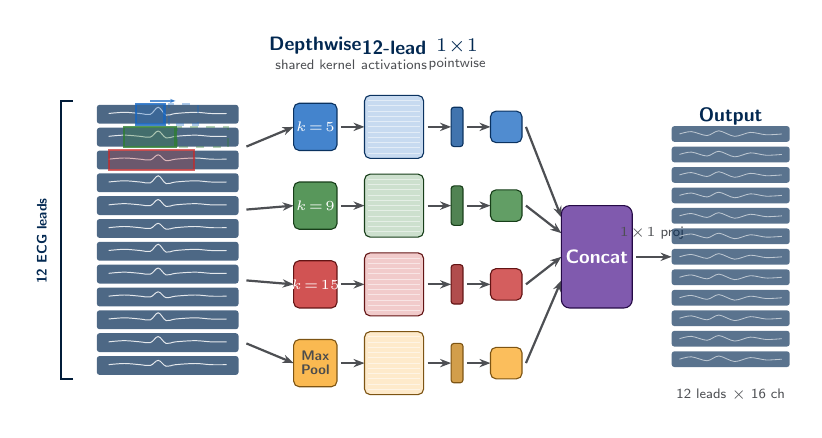
\begin{tikzpicture}[
    x=1cm, y=1cm,
    arr/.style={-{Stealth[length=4pt]}, thick, coolgray},
    lbl/.style={font=\scriptsize\bfseries, text=aggieblue, align=center},
    sublbl/.style={font=\tiny, text=coolgray, align=center},
  ]
    \definecolor{br1}{HTML}{1565C0}
    \definecolor{br2}{HTML}{2E7D32}
    \definecolor{br3}{HTML}{C62828}
    \definecolor{br4}{HTML}{F9A825}
    \definecolor{outc}{HTML}{4A148C}

    % ===== INPUT: 12 ECG lead bars with waveforms =====
    \foreach \i in {0,...,11}{
      \pgfmathsetmacro{\ypos}{\i * 0.29}
      \pgfmathsetmacro{\ymid}{\ypos + 0.13}
      \pgfmathsetmacro{\amp}{0.055 + mod(\i, 3) * 0.012}
      \fill[aggieblue, opacity=0.7, rounded corners=1pt] (0, \ypos) rectangle ++(1.8, 0.24);
      \draw[white, opacity=0.85, line width=0.35pt]
        plot[smooth, tension=0.6] coordinates {
          (0.15, \ymid)
          (0.35, {\ymid+0.015})
          (0.55, \ymid)
          (0.68, {\ymid-0.01})
          (0.78, {\ymid+\amp})
          (0.88, {\ymid-0.02})
          (1.0,  \ymid)
          (1.25, {\ymid+0.015})
          (1.45, \ymid)
          (1.65, \ymid)
        };
    }

    % --- Kernel windows superimposed on leads ---
    % k=5 on Lead I (index 11): narrow blue window + ghost showing slide
    \fill[br1, opacity=0.3] (0.5, {11*0.29-0.01}) rectangle ++(0.36, 0.26);
    \draw[br1, thick, opacity=0.8] (0.5, {11*0.29-0.01}) rectangle ++(0.36, 0.26);
    \draw[br1, dashed, thick, opacity=0.35] (0.92, {11*0.29-0.01}) rectangle ++(0.36, 0.26);
    \draw[-{Stealth[length=2pt]}, br1, thick, opacity=0.7]
      (0.68, {11*0.29+0.29}) -- ++(0.32, 0);

    % k=9 on Lead II (index 10): medium green window
    \fill[br2, opacity=0.3] (0.35, {10*0.29-0.01}) rectangle ++(0.65, 0.26);
    \draw[br2, thick, opacity=0.8] (0.35, {10*0.29-0.01}) rectangle ++(0.65, 0.26);
    \draw[br2, dashed, thick, opacity=0.35] (1.02, {10*0.29-0.01}) rectangle ++(0.65, 0.26);

    % k=15 on Lead III (index 9): wide red window
    \fill[br3, opacity=0.25] (0.15, {9*0.29-0.01}) rectangle ++(1.08, 0.26);
    \draw[br3, thick, opacity=0.7] (0.15, {9*0.29-0.01}) rectangle ++(1.08, 0.26);

    % Lead labels
    \node[font=\fontsize{3.5}{4}\selectfont\bfseries, text=white, anchor=east]
      at (-0.08, {11*0.29+0.13}) {I};
    \node[font=\fontsize{3.5}{4}\selectfont\bfseries, text=white, anchor=east]
      at (-0.08, {10*0.29+0.13}) {II};
    \node[font=\fontsize{3.5}{4}\selectfont\bfseries, text=white, anchor=east]
      at (-0.08, {9*0.29+0.13}) {III};
    \node[font=\fontsize{3.5}{4}\selectfont\bfseries, text=white, anchor=east]
      at (-0.08, {5*0.29+0.13}) {V1};
    \node[font=\fontsize{3.5}{4}\selectfont\bfseries, text=white, anchor=east]
      at (-0.08, {0*0.29+0.13}) {V6};
    % Bracket
    \draw[aggieblue!70!black, thick] (-0.3, -0.05) -- (-0.45, -0.05)
      -- (-0.45, {11*0.29+0.24+0.05}) -- (-0.3, {11*0.29+0.24+0.05});
    \node[font=\fontsize{4}{5}\selectfont\bfseries, text=aggieblue, rotate=90]
      at (-0.7, 1.7) {12 ECG leads};

    % ===== FOUR BRANCHES with full intermediate steps =====
    % Arrows from input to branches
    \draw[arr] (1.9, 2.9) -- (2.5, 3.15);
    \draw[arr] (1.9, 2.1) -- (2.5, 2.15);
    \draw[arr] (1.9, 1.2) -- (2.5, 1.15);
    \draw[arr] (1.9, 0.4) -- (2.5, 0.15);

    % --- Branch 1: k=5 ---
    % Depthwise kernel
    \fill[br1, opacity=0.8, rounded corners=2pt] (2.5, 2.85) rectangle ++(0.55, 0.6);
    \draw[br1!50!black, rounded corners=2pt] (2.5, 2.85) rectangle ++(0.55, 0.6);
    \node[font=\fontsize{5}{6}\selectfont\bfseries, text=white] at (2.775, 3.15) {$k\!=\!5$};
    \draw[arr] (3.1, 3.15) -- (3.4, 3.15);
    % 12-lead activations
    \fill[br1!40!white, opacity=0.6, rounded corners=2pt] (3.4, 2.75) rectangle ++(0.75, 0.8);
    \draw[br1!50!black, rounded corners=2pt] (3.4, 2.75) rectangle ++(0.75, 0.8);
    \foreach \j in {1,...,11}{
      \pgfmathsetmacro{\ly}{2.75 + \j * 0.8/12}
      \draw[white, opacity=0.5] (3.44, \ly) -- ++(0.67, 0);
    }
    \draw[arr] (4.2, 3.15) -- (4.5, 3.15);
    % Pointwise 1x1
    \fill[br1!80!black, opacity=0.8, rounded corners=1pt] (4.5, 2.9) rectangle ++(0.15, 0.5);
    \draw[br1!50!black, rounded corners=1pt] (4.5, 2.9) rectangle ++(0.15, 0.5);
    \draw[arr] (4.7, 3.15) -- (5.0, 3.15);
    % Branch output
    \fill[br1, opacity=0.75, rounded corners=2pt] (5.0, 2.95) rectangle ++(0.4, 0.4);
    \draw[br1!50!black, rounded corners=2pt] (5.0, 2.95) rectangle ++(0.4, 0.4);

    % --- Branch 2: k=9 ---
    \fill[br2, opacity=0.8, rounded corners=2pt] (2.5, 1.85) rectangle ++(0.55, 0.6);
    \draw[br2!50!black, rounded corners=2pt] (2.5, 1.85) rectangle ++(0.55, 0.6);
    \node[font=\fontsize{5}{6}\selectfont\bfseries, text=white] at (2.775, 2.15) {$k\!=\!9$};
    \draw[arr] (3.1, 2.15) -- (3.4, 2.15);
    \fill[br2!40!white, opacity=0.6, rounded corners=2pt] (3.4, 1.75) rectangle ++(0.75, 0.8);
    \draw[br2!50!black, rounded corners=2pt] (3.4, 1.75) rectangle ++(0.75, 0.8);
    \foreach \j in {1,...,11}{
      \pgfmathsetmacro{\ly}{1.75 + \j * 0.8/12}
      \draw[white, opacity=0.5] (3.44, \ly) -- ++(0.67, 0);
    }
    \draw[arr] (4.2, 2.15) -- (4.5, 2.15);
    \fill[br2!80!black, opacity=0.8, rounded corners=1pt] (4.5, 1.9) rectangle ++(0.15, 0.5);
    \draw[br2!50!black, rounded corners=1pt] (4.5, 1.9) rectangle ++(0.15, 0.5);
    \draw[arr] (4.7, 2.15) -- (5.0, 2.15);
    \fill[br2, opacity=0.75, rounded corners=2pt] (5.0, 1.95) rectangle ++(0.4, 0.4);
    \draw[br2!50!black, rounded corners=2pt] (5.0, 1.95) rectangle ++(0.4, 0.4);

    % --- Branch 3: k=15 ---
    \fill[br3, opacity=0.8, rounded corners=2pt] (2.5, 0.85) rectangle ++(0.55, 0.6);
    \draw[br3!50!black, rounded corners=2pt] (2.5, 0.85) rectangle ++(0.55, 0.6);
    \node[font=\fontsize{5}{6}\selectfont\bfseries, text=white] at (2.775, 1.15) {$k\!=\!15$};
    \draw[arr] (3.1, 1.15) -- (3.4, 1.15);
    \fill[br3!40!white, opacity=0.6, rounded corners=2pt] (3.4, 0.75) rectangle ++(0.75, 0.8);
    \draw[br3!50!black, rounded corners=2pt] (3.4, 0.75) rectangle ++(0.75, 0.8);
    \foreach \j in {1,...,11}{
      \pgfmathsetmacro{\ly}{0.75 + \j * 0.8/12}
      \draw[white, opacity=0.5] (3.44, \ly) -- ++(0.67, 0);
    }
    \draw[arr] (4.2, 1.15) -- (4.5, 1.15);
    \fill[br3!80!black, opacity=0.8, rounded corners=1pt] (4.5, 0.9) rectangle ++(0.15, 0.5);
    \draw[br3!50!black, rounded corners=1pt] (4.5, 0.9) rectangle ++(0.15, 0.5);
    \draw[arr] (4.7, 1.15) -- (5.0, 1.15);
    \fill[br3, opacity=0.75, rounded corners=2pt] (5.0, 0.95) rectangle ++(0.4, 0.4);
    \draw[br3!50!black, rounded corners=2pt] (5.0, 0.95) rectangle ++(0.4, 0.4);

    % --- Branch 4: MaxPool ---
    \fill[br4, opacity=0.8, rounded corners=2pt] (2.5, -0.15) rectangle ++(0.55, 0.6);
    \draw[br4!50!black, rounded corners=2pt] (2.5, -0.15) rectangle ++(0.55, 0.6);
    \node[font=\fontsize{4.5}{5}\selectfont\bfseries, text=black!70, align=center]
      at (2.775, 0.15) {Max\\Pool};
    \draw[arr] (3.1, 0.15) -- (3.4, 0.15);
    \fill[br4!40!white, opacity=0.6, rounded corners=2pt] (3.4, -0.25) rectangle ++(0.75, 0.8);
    \draw[br4!50!black, rounded corners=2pt] (3.4, -0.25) rectangle ++(0.75, 0.8);
    \foreach \j in {1,...,11}{
      \pgfmathsetmacro{\ly}{-0.25 + \j * 0.8/12}
      \draw[white, opacity=0.5] (3.44, \ly) -- ++(0.67, 0);
    }
    \draw[arr] (4.2, 0.15) -- (4.5, 0.15);
    \fill[br4!80!black, opacity=0.8, rounded corners=1pt] (4.5, -0.1) rectangle ++(0.15, 0.5);
    \draw[br4!50!black, rounded corners=1pt] (4.5, -0.1) rectangle ++(0.15, 0.5);
    \draw[arr] (4.7, 0.15) -- (5.0, 0.15);
    \fill[br4, opacity=0.75, rounded corners=2pt] (5.0, -0.05) rectangle ++(0.4, 0.4);
    \draw[br4!50!black, rounded corners=2pt] (5.0, -0.05) rectangle ++(0.4, 0.4);

    % Column labels above branches
    \node[lbl, above] at (2.775, 3.95) {Depthwise};
    \node[sublbl, above] at (2.775, 3.75) {shared kernel};
    \node[lbl, above] at (3.775, 3.95) {12-lead};
    \node[sublbl, above] at (3.775, 3.75) {activations};
    \node[lbl, above] at (4.575, 3.95) {$1\!\times\!1$};
    \node[sublbl, above] at (4.575, 3.75) {pointwise};

    % ===== CONCAT =====
    \draw[arr] (5.45, 3.15) -- (5.9, 2.0);
    \draw[arr] (5.45, 2.15) -- (5.9, 1.8);
    \draw[arr] (5.45, 1.15) -- (5.9, 1.5);
    \draw[arr] (5.45, 0.15) -- (5.9, 1.2);

    \fill[outc, opacity=0.7, rounded corners=3pt] (5.9, 0.85) rectangle ++(0.9, 1.3);
    \draw[outc!50!black, rounded corners=3pt] (5.9, 0.85) rectangle ++(0.9, 1.3);
    \node[font=\scriptsize\bfseries, text=white, align=center] at (6.35, 1.5) {Concat};

    % ===== 1x1 projection =====
    \draw[arr] (6.85, 1.5) -- (7.3, 1.5);
    \node[sublbl, above] at (7.05, 1.6) {$1\!\times\!1$ proj};

    % ===== OUTPUT: 12 lead bars with activation patterns =====
    \foreach \i in {0,...,11}{
      \pgfmathsetmacro{\ypos}{0.1 + \i * 0.26}
      \pgfmathsetmacro{\ymid}{\ypos + 0.1}
      \fill[aggieblue, opacity=0.65, rounded corners=1pt] (7.3, \ypos) rectangle ++(1.5, 0.2);
      \draw[white, opacity=0.6, line width=0.3pt]
        plot[smooth, tension=0.5] coordinates {
          ({7.3+0.1}, \ymid)
          ({7.3+0.25}, {\ymid+0.03})
          ({7.3+0.45}, {\ymid-0.02})
          ({7.3+0.6}, {\ymid+0.04})
          ({7.3+0.8}, {\ymid-0.03})
          ({7.3+1.0}, {\ymid+0.02})
          ({7.3+1.2}, {\ymid-0.01})
          ({7.3+1.4}, \ymid)
        };
    }
    \node[lbl, above] at (8.05, 3.05) {Output};
    \node[sublbl, below] at (8.05, -0.05) {12 leads $\times$ 16 ch};

  \end{tikzpicture}

  \vspace{0.3em}
  {\usebeamerfont{footline}\color{coolgray}
  Shared kernel slides along each lead independently \textbullet{}
  $1\!\times\!1$ pointwise mixes channels \textbullet{}
  $\sim\!k\!\times$ fewer params}
\end{frame}

% ---------- Subsection Slide: Squeeze-Excitation ----------
\begin{frame}{Neural Network Modeling --- Squeeze-Excitation (SE) Block}
  \begin{columns}[T]

    \begin{column}{0.48\textwidth}
      {\small\Raleway\bfseries\color{aggieblue} Mechanism (Hu et al., 2018)}\\[0.4em]
      \usebeamerfont{footline}\color{coolgray}
      Adaptive channel recalibration in three steps:\\[0.3em]

      \textbf{1.\ Squeeze} --- Global average pooling compresses each channel to a scalar:
      \[
        z_c = \frac{1}{T}\sum_{t=1}^{T} x_c(t)
      \]

      \textbf{2.\ Excite} --- Two FC layers learn channel interdependencies:
      \[
        \mathbf{s} = \sigma\!\bigl(W_2 \cdot \text{ReLU}(W_1 \cdot \mathbf{z})\bigr)
      \]
      $W_1 \in \mathbb{R}^{C/r \times C}$, $W_2 \in \mathbb{R}^{C \times C/r}$, reduction $r=4$

      \vspace{0.3em}
      \textbf{3.\ Scale} --- Channel-wise multiplication:
      \[
        \tilde{x}_c = s_c \cdot x_c
      \]
    \end{column}

    \begin{column}{0.48\textwidth}
      {\small\Raleway\bfseries\color{aggieblue} Role in RepNet-SE}\\[0.4em]
      \usebeamerfont{footline}\color{coolgray}
      Placed after each conv block, before cross-lead attention:\\[0.3em]

      \begin{beamercolorbox}[wd=\textwidth,rounded=true,leftskip=0.5em,rightskip=0.5em,sep=0.4em]{boxgray}
        \scriptsize\Lato\color{coolgray}
        \textbf{Stage 1:} MultiScaleDSConv(1$\to$16) + \textbf{SE(16)}\\
        \textbf{Stage 2:} DSConvBlock(16$\to$32) + \textbf{SE(32)}\\
        \textbf{Stage 3:} DSConvBlock(32$\to$64) + \textbf{SE(64)}\\[0.3em]
        Fusion: per-lead GAP $\to$ LeadAttentionPool $\to$ Linear(64$\to$2)
      \end{beamercolorbox}

      \vspace{0.5em}
      {\small\Raleway\bfseries\color{aggieblue} Why SE for ECG?}\\[0.3em]
      \begin{itemize}
        \item Learned feature maps mix morphological cues (P/T amplitude, ST segment, QRS width)
        \item SE suppresses noisy channels and amplifies discriminative ones \textit{per lead, per sample}
        \item IncepSE (2023) showed +0.013 AUROC over vanilla InceptionTime on ECG tasks
        \item Minimal overhead: only $2C^2/r$ extra parameters per block
      \end{itemize}
    \end{column}

  \end{columns}
\end{frame}

% ---------- Subsection Slide: Multi-Head Cross-Lead Attention ----------
\begin{frame}{Neural Network Modeling --- Multi-Head Cross-Lead Attention}
  \begin{columns}[T]

    \begin{column}{0.48\textwidth}
      {\small\Raleway\bfseries\color{aggieblue} Multi-Head Self-Attention}\\[0.4em]
      \usebeamerfont{footline}\color{coolgray}
      Each of 12 leads is pooled to a $C$-dimensional token. Attention operates over these tokens:\\[0.3em]

      \textbf{Scaled Dot-Product Attention:}
      \[
        \text{Attn}(Q,K,V) = \text{softmax}\!\Bigl(\frac{QK^\top}{\sqrt{d_k}}\Bigr)\!V
      \]
      \textbf{Multi-Head} ($h=4$ heads): each head learns different lead relationships, then outputs are concatenated and projected.\\[0.3em]

      \begin{beamercolorbox}[wd=\textwidth,rounded=true,leftskip=0.5em,rightskip=0.5em,sep=0.3em]{boxgray}
        \scriptsize\Lato\color{coolgray}
        \textbf{Example learned patterns:}\\
        Lead~II $\leftrightarrow$ V4 (inferior--precordial),\\
        aVR $\leftrightarrow$ V1 (right-heart axis),\\
        aVL $\leftrightarrow$ III (lateral--inferior)
      \end{beamercolorbox}
    \end{column}

    \begin{column}{0.48\textwidth}
      {\small\Raleway\bfseries\color{aggieblue} Gated Cross-Lead Mechanism}\\[0.4em]
      \usebeamerfont{footline}\color{coolgray}
      After attention, a \textbf{gating layer} modulates each lead's feature map:\\[0.3em]

      \begin{enumerate}
        \item \textbf{Pool} each lead's $(C, T)$ map to a $C$-dim token via adaptive average pooling
        \item \textbf{Attend} across 12 lead tokens with multi-head attention + residual + LayerNorm
        \item \textbf{Gate} $= \sigma(\text{FC}(\text{attn\_out}))$ produces per-lead, per-channel weights in $[0, 1]$
        \item \textbf{Scale} original feature map: $\tilde{x}_\ell = x_\ell \odot g_\ell$
      \end{enumerate}

      \vspace{0.4em}
      {\small\Raleway\bfseries\color{aggieblue} Architecture Placement}\\[0.3em]
      \begin{beamercolorbox}[wd=\textwidth,rounded=true,leftskip=0.5em,rightskip=0.5em,sep=0.3em]{boxgray}
        \scriptsize\Lato\color{coolgray}
        Applied \textbf{after every stage}, allowing the model to learn cross-lead dependencies at multiple abstraction levels:\\[0.2em]
        Stage~1 (16-ch): low-level morphology\\
        Stage~2 (32-ch): interval features\\
        Stage~3 (64-ch): high-level patterns\\[0.2em]
        Final fusion via \textbf{LeadAttentionPool}: learned softmax weighting over 12 lead embeddings $\to$ single patient vector.
      \end{beamercolorbox}
    \end{column}

  \end{columns}
\end{frame}

% ---------- Subsection Slide: Model Performance ----------
\begin{frame}{Neural Network Modeling --- Model Performance}
  \begin{columns}[T]

    \begin{column}{0.48\textwidth}
      \centering
      {\small\Raleway\bfseries\color{aggieblue} 20-Seed Cross-Validation (5-Bag Ensemble)}\\[0.4em]
      \resizebox{\textwidth}{!}{%
        \begin{tabular}{lcc}
          \toprule
          \textbf{Metric} & \textbf{Mean $\pm$ Std} & \textbf{Best Seed} \\
          \midrule
          AUROC & $0.668 \pm 0.066$ & 0.787 \\
          AUPRC & $0.291 \pm 0.060$ & 0.450 \\
          Brier Score & $0.225 \pm 0.056$ & 0.141 \\
          Sens @ Sp$\geq$80\% & $0.432 \pm 0.085$ & 0.582 \\
          \bottomrule
        \end{tabular}
      }%

      \vspace{0.5em}
      {\small\Raleway\bfseries\color{aggieblue} Configuration Explored}\\[0.3em]
      \usebeamerfont{footline}\color{coolgray}
      \resizebox{\textwidth}{!}{%
        \begin{tabular}{ll}
          \toprule
          \textbf{Property} & \textbf{Value} \\
          \midrule
          Best config & \texttt{repnet\_se\_deep} \\
          Stages & 4 (16$\to$32$\to$48$\to$64) \\
          Total params & 65{,}748 \\
          Bags per seed & 5 (prob.\ averaged) \\
          Splits & StratifiedGroupKFold ($k=5$) \\
          \bottomrule
        \end{tabular}
      }%
    \end{column}

    \begin{column}{0.48\textwidth}
      \centering
      {\small\Raleway\bfseries\color{aggieblue} ROC \& Precision-Recall Curves}\\[0.3em]
      \begin{beamercolorbox}[wd=\textwidth,rounded=true,leftskip=0.1em,rightskip=0.1em,sep=0.1em]{boxgray}
        \centering
        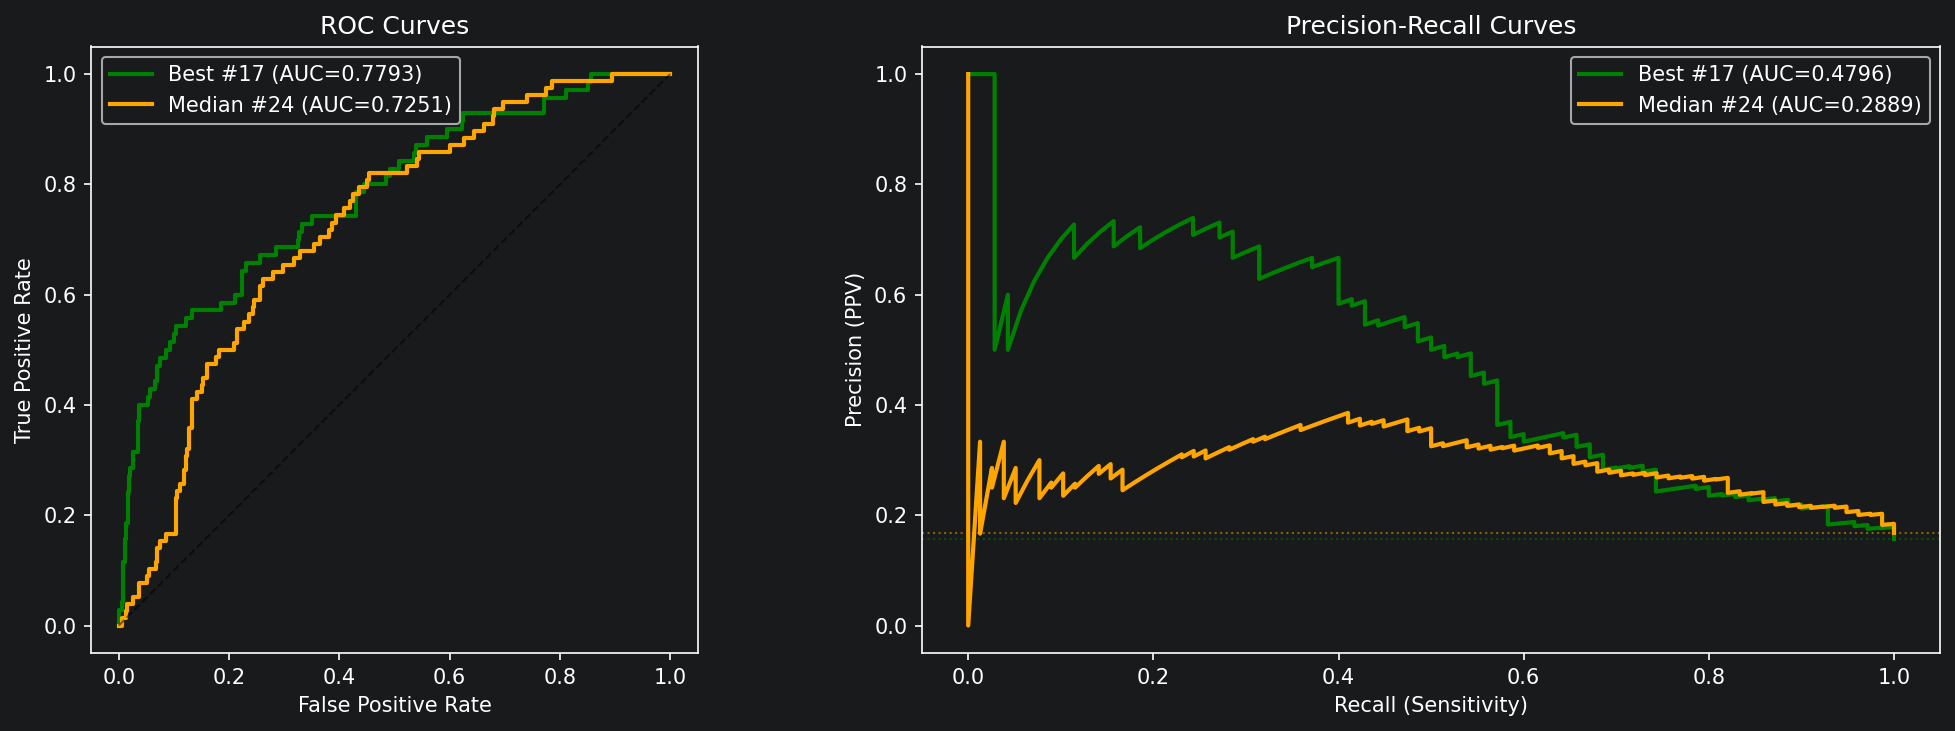
\includegraphics[width=0.96\textwidth,height=3.2cm,keepaspectratio]{roc_pr_curves.png}
      \end{beamercolorbox}

      \vspace{0.4em}
      \begin{beamercolorbox}[wd=\textwidth,rounded=true,leftskip=0.5em,rightskip=0.5em,sep=0.3em]{boxgray}
        \scriptsize\Lato\color{coolgray}
        \textbf{Variance note:} High seed-to-seed variance (AUROC 0.58--0.79) reflects the small positive class ($n=67$ PE+ in test). Bagging (5 models averaged) and config exploration (8 configs scouted $\to$ best selected) partially mitigate this.
      \end{beamercolorbox}
    \end{column}

  \end{columns}
\end{frame}

% ---------- Subsection Slide: Interpretability --- Saliency ----------
\begin{frame}{Neural Network Modeling --- Saliency Maps}
  \begin{columns}[T]

    \begin{column}{0.42\textwidth}
      {\small\Raleway\bfseries\color{aggieblue} Gradient-Based Attribution}\\[0.4em]
      \usebeamerfont{footline}\color{coolgray}
      \textbf{Method:} Compute $\frac{\partial \hat{y}_{\text{PE+}}}{\partial x_{\ell,t}}$ --- the gradient of the PE-positive logit w.r.t.\ each sample point across all 12 leads.\\[0.3em]

      Regions with high gradient magnitude are the time points the model relies on most for its prediction.\\[0.4em]

      {\small\Raleway\bfseries\color{aggieblue} Clinical Observations}\\[0.3em]
      \begin{itemize}
        \item High saliency around \textbf{P-wave onset} and \textbf{T-wave peak} --- consistent with known PE-associated repolarization changes
        \item \textbf{ST segment} contributes in true-positive cases
        \item Lead~II and precordial leads (V3--V5) show the strongest attribution signals
      \end{itemize}
    \end{column}

    \begin{column}{0.54\textwidth}
      \centering
      {\small\Raleway\bfseries\color{aggieblue} Saliency Overlay --- Lead~II}\\[0.3em]
      \begin{beamercolorbox}[wd=\textwidth,rounded=true,leftskip=0.1em,rightskip=0.1em,sep=0.1em]{boxgray}
        \centering
        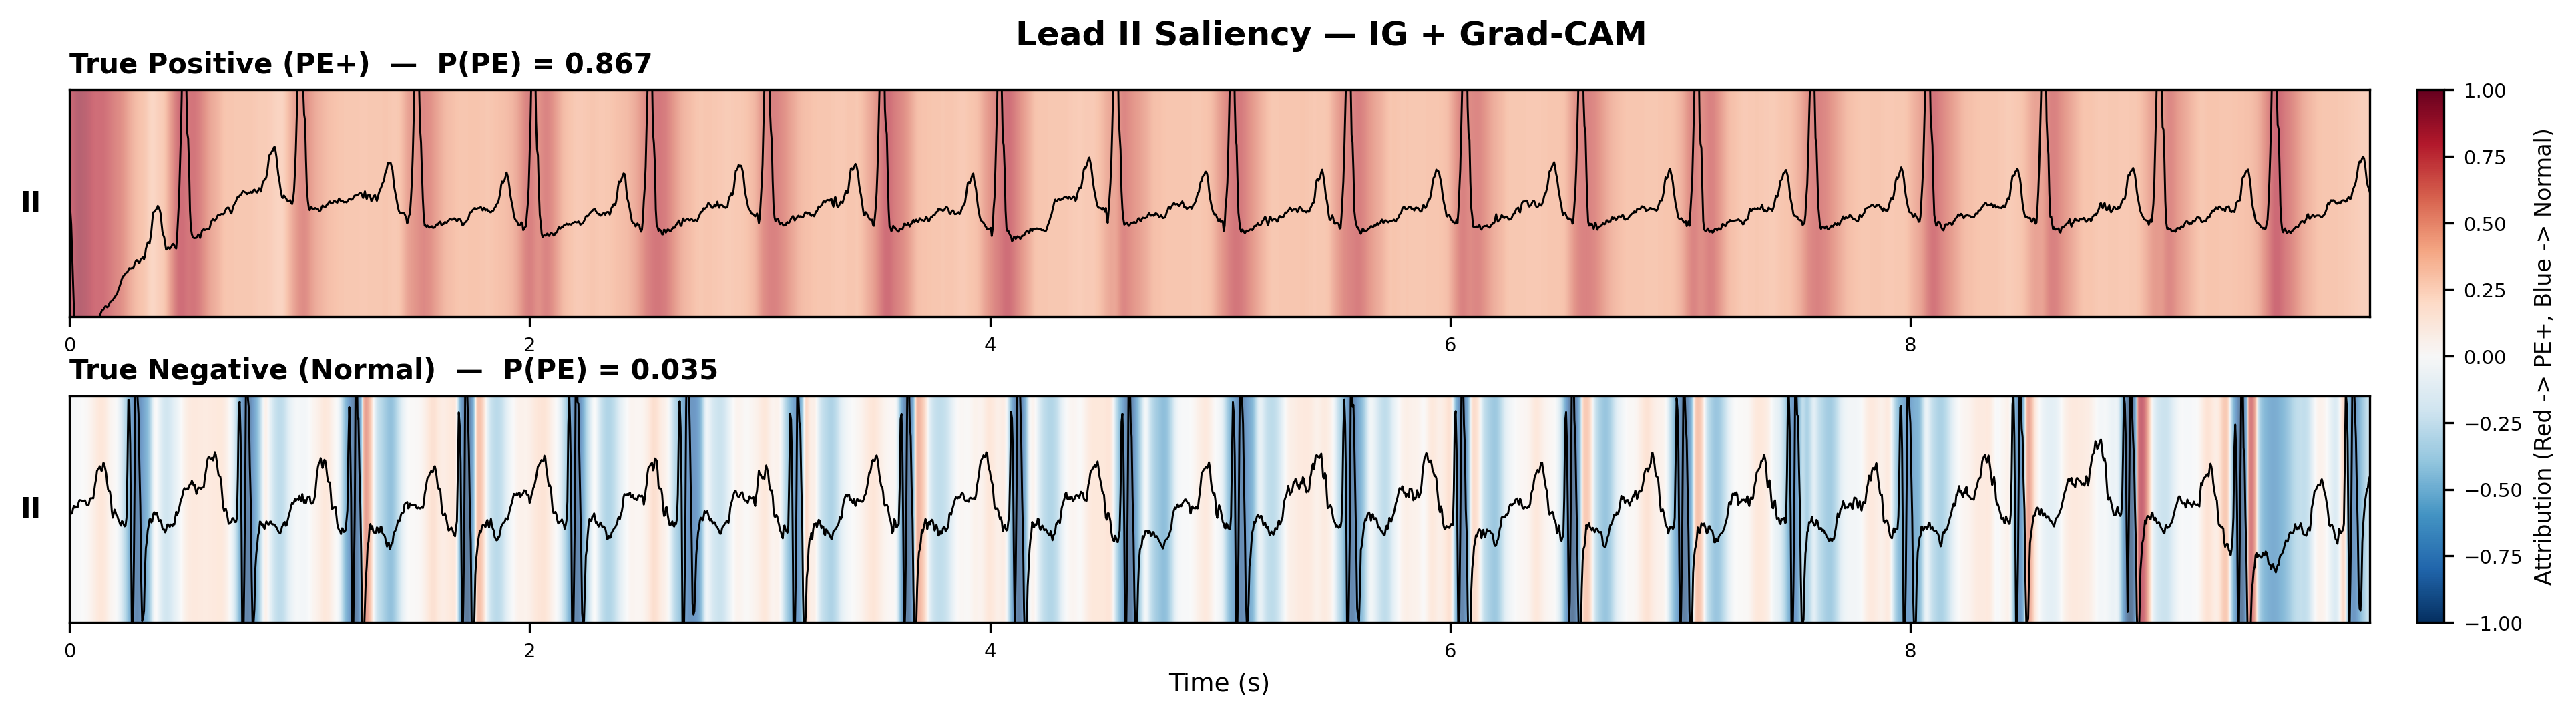
\includegraphics[width=0.98\textwidth,height=4.4cm,keepaspectratio]{saliency_poster_lead_II.png}
      \end{beamercolorbox}
      \vspace{0.3em}
      {\scriptsize\Lato\color{coolgray} Top: confident true-positive (PE+). Bottom: confident true-negative (PE$-$). Color intensity $\propto$ gradient magnitude. The model attends to distinct morphological regions for each class.}
    \end{column}

  \end{columns}
\end{frame}

% ---------- Conclusion Slide ----------
\begin{frame}{Conclusion}
  \begin{columns}[T]

    \begin{column}{0.48\textwidth}
      {\small\Raleway\bfseries\color{aggieblue} Key Findings}\\[0.4em]
      \usebeamerfont{footline}\color{coolgray}
      \begin{itemize}
        \item Both approaches detect a \textbf{preeclampsia signal} in standard 12-lead ECGs
        \item Decision-tree ensemble achieves \textbf{AUROC 75.7} (Unweighted Voting+) with handcrafted features
        \item Neural network (RepNet-SE) achieves \textbf{AUROC 66.8} mean / \textbf{78.7} best seed from raw waveforms alone
        \item Feature-based models more \textbf{stable} across data splits; neural models show higher variance but stronger peaks
      \end{itemize}

      \vspace{0.3em}
      \begin{beamercolorbox}[wd=\textwidth,rounded=true,leftskip=0.5em,rightskip=0.5em,sep=0.3em]{boxgray}
        \scriptsize\Lato\color{coolgray}
        \textbf{Complementary strengths:} Feature engineering reveals \textit{which} ECG characteristics matter (Tp-e, QRS-T angle); neural models learn directly from morphology without manual feature design.
      \end{beamercolorbox}
    \end{column}

    \begin{column}{0.48\textwidth}
      {\small\Raleway\bfseries\color{aggieblue} Comparison Summary}\\[0.4em]
      \resizebox{\textwidth}{!}{%
        \begin{tabular}{lcc}
          \toprule
          & \textbf{Decision-Tree} & \textbf{Neural (RepNet-SE)} \\
          \midrule
          Input & 191 features & Raw 12-lead ECG \\
          Best AUROC & 75.7 & 78.7 (best seed) \\
          Mean AUROC & $74.5 \pm 3.9$ & $66.8 \pm 6.6$ \\
          Stability & Higher & Lower \\
          Interpretability & Direct & Saliency maps \\
          Feature eng.\ & Required & None \\
          Params & N/A & 65{,}748 \\
          \bottomrule
        \end{tabular}
      }%

      \vspace{0.5em}
      {\small\Raleway\bfseries\color{aggieblue} Takeaway}\\[0.3em]
      \usebeamerfont{footline}\color{coolgray}
      ECG-based preeclampsia screening is \textbf{feasible} with either approach. The small positive class ($n=335$ PE+) is the primary limiting factor --- larger datasets would narrow the gap between mean and best-seed neural performance.
    \end{column}

  \end{columns}
\end{frame}

% ---------- Future Work Slide ----------
\begin{frame}{Future Work}
  \begin{columns}[T]

    \begin{column}{0.48\textwidth}
      {\small\Raleway\bfseries\color{aggieblue} Data \& Validation}\\[0.4em]
      \usebeamerfont{footline}\color{coolgray}
      \begin{itemize}
        \item \textbf{Larger, multi-site datasets} to reduce variance and improve generalizability
        \item \textbf{Prospective validation} on newly collected ECGs to test real-world performance
        \item \textbf{Temporal analysis:} ECGs at multiple gestational time points to study when PE becomes detectable
        \item \textbf{Subgroup analysis} by PE severity (mild vs.\ severe) and gestational age at onset
      \end{itemize}
    \end{column}

    \begin{column}{0.48\textwidth}
      {\small\Raleway\bfseries\color{aggieblue} Modeling \& Deployment}\\[0.4em]
      \usebeamerfont{footline}\color{coolgray}
      \begin{itemize}
        \item \textbf{Hybrid ensemble:} combine handcrafted features with neural waveform representations for a single, stronger classifier
        \item \textbf{Self-supervised pretraining} on large unlabeled ECG corpora (e.g.\ PhysioNet) before fine-tuning on PE task
        \item \textbf{Lightweight deployment:} quantize RepNet-SE ($\sim$65K params) for edge devices or bedside monitors
        \item \textbf{Clinical decision support:} integrate saliency maps into physician-facing reports for explainable risk scores
      \end{itemize}
    \end{column}

  \end{columns}
\end{frame}

% ---------- Closing Slide ----------
{%
  \setbeamertemplate{footline}{}%
  \begin{frame}[plain,noframenumbering]
    \begin{tikzpicture}[remember picture,overlay]
      \fill[aggieblue] (current page.south west) rectangle (current page.north east);
    \end{tikzpicture}
    \vfill
    \centering
    {\Raleway\bfseries\Huge\color{white} Thank you}\\[0.6em]
    {\color{aggiegold}\rule{4cm}{0.06cm}}\\[0.8em]
    {\Lato\large\color{white} Questions?}
    \vfill
  \end{frame}
}

\end{document}